\documentclass[pra,12pt]{revtex4}
\usepackage{amsmath}
\usepackage{amssymb}
\usepackage{graphicx}
\usepackage{color}
\usepackage{mathrsfs}
\usepackage{enumerate}
\usepackage{epigraph}
\usepackage{framed}
\usepackage[pdfborder={0 0 0},colorlinks=true,linkcolor=blue,urlcolor=blue]{hyperref}

\def\ket#1{\left|#1\right\rangle}
\def\bra#1{\left\langle#1\right|}
\def\braket#1{\left\langle#1\right\rangle}

\usepackage{fancyhdr}
\fancyhf{}
\lhead{\tiny Y.~D.~Chong}
\rhead{\scriptsize PH4401: Quantum Mechanics III}
\lfoot{}
\rfoot{\thepage}
\pagestyle{fancy}

\setlength{\parindent}{14pt}
\renewcommand{\theequation}{4.\arabic{equation}}

\renewcommand{\baselinestretch}{1.0}
\setlength{\parskip}{0.07in}
\setlength{\epigraphwidth}{.6\textwidth}

\begin{document}

\begin{center}
{\Large \textbf{Chapter 4: Quantum Electrodynamics}}
\end{center}

This chapter provides a survey of \textbf{quantum electrodynamics},
the quantum theory of the electromagnetic field and its interactions
with electrons and other electrically charged particles.  We start by
formulating Hamiltonians to describe how a quantum mechanical electron
is affected by classical electromagnetic fields.  Next, we describe
the quantization of Maxwell's equations, which yields a quantum field
theory in which the elementary excitations are photons---particles of
light.  The last step is to formulate a theory in which both electrons
and photons are treated on the same footing, as excitations of
underlying quantum fields.  Along the way, we will see how relativity
can be accomodated with quantum mechanics.

Quantum electrodynamics is a rich and intricate theory, and we will
not be able to cover many important areas, such as the detailed
relationship with special relativity or diagrammatic methods for
performing field theoretical calculations.  For further reading, two
recommended texts are Dyson's 1951 lecture notes
(\hyperref[cite:dyson]{Dyson 1951}) and Zee's introductory textbook
\textit{Quantum Field Theory in a Nutshell} (\hyperref[cite:zee]{Zee
  2010}).

\section{Quantization of the Lorentz Force Law}

\subsection{Non-relativistic electrons in an electromagnetic field}
\label{sec:nonrel}

Consider a non-relativistic charged particle in an electromagnetic
field.  As we are mainly interested in the physics of electrons
interacting with electromagnetic fields, we henceforth take the
electric charge of the particle to be $-e$, where $e =
1.602\times10^{-19}\,\mathrm{C}$ is the elementary charge.  To
describe particles with an arbitrary electric charge $q$, simply
perform the substitution $e \rightarrow -q$ in all formulas in the
rest of this chapter.

We begin by formulating the Hamiltonian governing the quantum dynamics
of such a particle, subject to two simplifying assumptions: (i) the
particle has charge and mass but is otherwise ``featureless'' (i.e.,
unlike a real electron, it has no spin angular momentum, and no
magnetic dipole moment), and (ii) the electromagnetic field is treated
as a classical field (i.e., the electric and magnetic fields are
definite quantities).  We will show how to drop these simplifications
in subsequent sections.

In the classical regime, the action of an electromagnetic field on a
point charged particle is decribed by the Lorentz force law,
\begin{equation}
  \mathbf{F}(\mathrm{r},t) = -e\Big(\mathbf{E}(\mathrm{r},t)
  + \dot{\mathbf{r}}\times \mathbf{B}(\mathrm{r},t)\Big),
\end{equation}
where $\mathbf{r}$ and $\dot{\mathbf{r}}$ respectively denote the
position and velocity of the particle, $t$ is the time, and
$\mathbf{E}$ and $\mathbf{B}$ are the electric and magnetic fields.
If there are no other forces acting on the particle, then according to
Newton's second law, the equation of motion is
\begin{equation}
  m\ddot{\mathbf{r}} = -e\Big(\mathbf{E}(\mathrm{r},t)
  + \dot{\mathbf{r}} \times \mathbf{B}(\mathrm{r},t)\Big),
  \label{eom}
\end{equation}
where $m$ is the particle's mass.  To quantize this, we must convert
the equation of motion into the form of Hamilton's equations of
motion.

Let us introduce the electromagnetic scalar and vector potentials
$\Phi(\mathrm{r},t)$ and $\mathbf{A}(\mathrm{r},t)$, where
\begin{align}
  \mathbf{E}(\mathbf{r},t) &= - \nabla \Phi(\mathbf{r},t) - \frac{\partial\mathbf{A}}{\partial t} \\
  \mathbf{B}(\mathbf{r},t) &= \nabla \times \mathbf{A}(\mathbf{r},t).
  \label{Bfield}
\end{align}
We now postulate that the equation of motion \eqref{eom} can be
described by the Lagrangian
\begin{framed}
\begin{equation}
  L(\mathbf{r},\dot{\mathbf{r}},t) = \frac{1}{2}m\dot{\mathbf{r}}^2
  + e \Big[\Phi(\mathbf{r},t) - \dot{\mathbf{r}} \cdot \mathbf{A}(\mathbf{r},t)
    \Big].
  \label{Lag}
\end{equation}
\end{framed}
\vskip -0.15in
\noindent
This is very similar to the usual prescription for the Lagrangian as
the kinetic energy minus the potential energy, with $-e\Phi$ serving
as the potential energy function.  However, there is an extra
$-e\dot{\mathbf{r}} \cdot \mathbf{A}$ term, which will turn out to be
responsible for the magnetic force.

We want to plug the Lagrangian \eqref{Lag} into the Euler-Lagrange
equations
\begin{equation}
  \frac{\partial L}{\partial r_i} = \frac{d}{dt}
  \frac{\partial L}{\partial \dot{r}_i}.
  \label{EulerLagrange}
\end{equation}
The partial derivatives of the Lagrangian are:
\begin{align}
  \begin{aligned}
    \frac{\partial L}{\partial r_i} &=
    e\Big[\partial_i \Phi - \dot{r}_j \,\partial_i A_j \Big]\\
    \frac{\partial L}{\partial \dot{r}_i} &= m\dot{r}_i - e A_i.
  \end{aligned}
\end{align}
Now we want to take the \textit{total} time derivative of $\partial L
/\partial \dot{r}_i$.  In doing so, note that the $\mathbf{A}$ field
has its own $t$-dependence, as well as varying with the particle's
$t$-dependent position.  Thus,
\begin{align}
  \begin{aligned}
    \frac{d}{dt} \frac{\partial L}{\partial \dot{r}_i}
    &= m\ddot{r}_i - e\, \frac{d}{dt} A_i(\mathbf{r}(t),t) \\
    &= m\ddot{r}_i - e\, \partial_t A_i
    - e\, \dot{r}_j \partial_j A_i.
  \end{aligned}
\end{align}
(In the above equations, $\partial_i \equiv \partial/\partial r_i$,
where $r_i$ is the $i$-th component of the position vector, while
$\partial_t \equiv \partial/\partial t$.)  Plugging these expressions
into the Euler-Lagrange equations \eqref{EulerLagrange} gives
\begin{align}
  \begin{aligned}
    m\ddot{r}_i &=
    -e\Big[\Big(-\partial_i \Phi - \partial_t A_i\Big)
      + \dot{r}_j \Big( \partial_i A_j - \partial_j A_i\Big) \Big] \\
    &= -e \Big[E_i(\mathbf{r},t) + \big(\dot{\mathbf{r}} \times
      \mathbf{B}(\mathbf{r},t) \big)_i\, \Big].
  \end{aligned}
\end{align}
(The last step can be derived by expressing the cross product using
the Levi-Cevita symbol, and using the identity $\varepsilon_{ijk}
\varepsilon_{lmk} = \delta_{il} \delta_{jm} - \delta_{im}
\delta_{jl}$.)  As desired, this is the equation of motion
corresponding to the Lorentz force.

We can now use the Lagrangian to derive the Hamiltonian.  The
canonical momentum is
\begin{equation}
  p_i = \frac{\partial L}{\partial \dot{r}_i} = m\dot{r}_i - e A_i.
  \label{canonp}
\end{equation}
The Hamiltonian is defined as $H(\mathbf{r},\mathbf{p}) = \mathbf{p}
\cdot \dot{\mathbf{r}} - L$, and we use Eq.~\eqref{canonp} to be
express it in terms of $\mathbf{p}$ rather than $\dot{\mathbf{r}}$:
\begin{align}
  \begin{aligned}
    H &= \mathbf{p}\cdot \left(\frac{\mathbf{p}+e\mathbf{A}}{m}\right)
    - \left(\frac{|\mathbf{p}+e\mathbf{A}|^2}{2m}
    + e\Phi - \frac{e}{m}(\mathbf{p}+e\mathbf{A})\cdot \mathbf{A}\right) \\
    &= \frac{|\mathbf{p}+e\mathbf{A}|^2}{m}
    - \frac{e}{m}\mathbf{A}\cdot \left(\mathbf{p}+e\mathbf{A}\right)
    - \left(\frac{|\mathbf{p}+e\mathbf{A}|^2}{2m}
    + e\Phi - \frac{e}{m}(\mathbf{p}+e\mathbf{A})\cdot \mathbf{A}\right).
  \end{aligned}
\end{align}
After cancelling various terms, we arrive at the result
\begin{framed}
  \begin{equation}
    H = \frac{|\mathbf{p}+e\mathbf{A}(\mathbf{r},t)|^2}{2m} - e\Phi(\mathbf{r},t).
  \end{equation}
\end{framed}
\vskip -0.15in
\noindent
This looks much like the familiar Hamiltonian for a non-relativistic
particle,
\begin{equation*}
  H = \frac{|\mathbf{p}|^2}{2m} + V(\mathbf{r},t).
\end{equation*}
The electromagnetic scalar potential $\Phi(\mathbf{r},t)$ acts like a
potential energy term, as might be expected.  More surprising is the
fact that the vector potential appears via the substitution
\begin{equation}
  \mathbf{p} \rightarrow \mathbf{p} + e\mathbf{A}(\mathbf{r},t).  
\end{equation}
What does this mean?

To answer this, think about what ``momentum'' means in the context of
a charged particle in an electromagnetic field.  Noether's theorem
states that every symmetry of a system (whether classical or quantum)
is associated with a conserved quantity.  Momentum is the quantity
conserved when the system is symmetric under spatial translations.  We
can see this from the Hamilton equation
\begin{equation*}
  \frac{dp_i}{dt} = \frac{\partial H}{\partial r_i},
\end{equation*}
which implies that if a Hamiltonian is $\mathbf{r}$-independent, then
$d\mathbf{p}/dt = 0$.  But when the electromagnetic potentials are
$\mathbf{r}$-independent, the quantity $m\dot{\mathbf{r}}$ (which we
usually call momentum) is \textit{not} necessarily conserved!
Consider the potentials
\begin{equation}
  \Phi(\mathbf{r}, t) = 0, \;\;\; \mathbf{A}(\mathbf{r}, t) = Ct \hat{z},
\end{equation}
where $C$ is some constant.  These potentials are evidently
$\mathbf{r}$-independent, but the vector potential is time-dependent,
so the $-\dot{\mathbf{A}}$ term in Eq.~\eqref{Bfield} gives a
non-vanishing electric field:
\begin{equation}
  \mathbf{E}(\mathbf{r},t) = - C\hat{z}, \;\;\;\mathbf{B}(\mathbf{r},t) = 0.
\end{equation}
The Lorentz force law then says that
\begin{equation}
  \frac{d}{dt}(m\dot{\mathbf{r}}) = eC\hat{z},
\end{equation}
and thus $m\dot{\mathbf{r}}$ is not conserved.  On the other hand, the
quantity $\mathbf{p} = m\dot{\mathbf{r}} - e \mathbf{A}$ \textit{is}
conserved:
\begin{equation}
  \frac{d}{dt}(m\dot{\mathbf{r}} - e\mathbf{A}) =
  eC\hat{z} - eC\hat{z} = 0.
\end{equation}
Hence, this quantity serves as appropriate canonical momentum for a
particle in an electromagnetic field.

The last step is to go from classical to quantum mechanics.  To do
this, we simply replace $\mathbf{r}$ with the position operator
$\hat{\mathbf{r}}$, and $\mathbf{p}$ with the momentum operator
$\hat{\mathbf{p}}$.  The resulting quantum Hamiltonian is
\begin{framed}
  \begin{equation}
    \hat{H}(t) = \frac{|\hat{\mathbf{p}}+e\mathbf{A}(\hat{\mathbf{r}},t)|^2}{2m}
    - e\Phi(\hat{\mathbf{r}},t).
    \label{quantumH}
  \end{equation}
\end{framed}
\vskip -0.15in
\noindent
Note: the momentum operator is $\hat{\mathbf{p}} = -i\hbar\nabla$
in the wavefunction representation, as usual.

\subsection{Gauge symmetry}
\label{sec:gauge}

The Hamiltonian \eqref{quantumH} possesses a subtle property known as
\textbf{gauge symmetry}.  Suppose we modify the scalar and vector
potentials via the substitutions
\begin{align}
  \begin{aligned}
    \Phi(\mathbf{r},t) &\rightarrow \Phi(\mathbf{r},t) - \dot{\Lambda}(\mathbf{r},t)\\
    \mathbf{A}(\mathbf{r},t) &\rightarrow
    \mathbf{A}(\mathbf{r},t) + \nabla{\Lambda}(\mathbf{r},t),
  \end{aligned}
\end{align}
where $\Lambda(\mathbf{r},t)$ is an arbitrary scalar field called a
\textbf{gauge field}.  This is the \textbf{gauge transformation} of
classical electromagnetism, which as we know leaves the electric and
magnetic fields unchanged.  When applied to the Hamiltonian
\eqref{quantumH}, it generates a new Hamiltonian,
\begin{equation}
  \hat{H}_\Lambda(t)
  = \frac{|\hat{\mathbf{p}}+e\mathbf{A}(\hat{\mathbf{r}},t) + e\nabla\Lambda(\hat{\mathbf{r}},t)|^2}{2m}
  - e\Phi(\hat{\mathbf{r}},t) + e\dot{\Lambda}(\hat{\mathbf{r}},t).
\end{equation}
If $\psi(\mathbf{r},t)$ is any wavefunction obeying the Schr\"odinger
equation for the original Hamiltonian,
\begin{equation}
  i\hbar\frac{\partial\psi}{\partial t} =
  \hat{H}(t) \psi(\mathbf{r},t)
  = \left[\frac{|\hat{\mathbf{p}}+e\mathbf{A}(\hat{\mathbf{r}},t)|^2}{2m}
  - e\Phi(\hat{\mathbf{r}},t) \right]\psi(\mathbf{r},t),
\end{equation}
then it can be shown that the wavefunction $\psi(\mathbf{r},t)
\exp(-ie\Lambda/\hbar)$ automatically satisfies the Schr\"odinger
equation for the transformed Hamiltonian:
\begin{equation}
  i\hbar\frac{\partial}{\partial t} \left[\psi(\mathbf{r},t) \, \exp\left(-\frac{ie\Lambda(\mathbf{r},t)}{\hbar}\right)\right] =
  \hat{H}_\Lambda(t) \left[\psi(\mathbf{r},t) \, \exp\left(-\frac{ie\Lambda(\mathbf{r},t)}{\hbar}\right)\right].
  \label{gaugeschrod}
\end{equation}

To prove this, observe how time and space derivatives act on the new
wavefunction:
\begin{align}
  \begin{aligned}
    \frac{\partial}{\partial t} \left[\psi \, \exp\left(-\frac{ie\Lambda}{\hbar}\right)\right] &=
    \left[\frac{\partial\psi}{\partial t} \;-\; \frac{ie}{\hbar} \dot{\Lambda}\, \psi
      \,\, \right] \exp\left(\frac{ie\Lambda}{\hbar}\right)\\
    \nabla \left[\psi \, \exp\left(-\frac{ie\Lambda}{\hbar}\right)\right] &=
    \left[\nabla \psi - \frac{ie}{\hbar} \nabla \Lambda \,\psi \right] \exp\left(\frac{ie\Lambda}{\hbar}\right).
  \end{aligned}
\end{align}
When the extra terms generated by the $\exp(ie\Lambda/\hbar)$ factor
are slotted into the Schr\"odinger equation, they cancel the gauge
terms in the scalar and vector potentials.  For example,
\begin{align}
  \Big(-i\hbar\nabla + e\mathbf{A} + e\nabla\Lambda\Big)
  \left[\psi \, \exp\left(-\frac{ie\Lambda}{\hbar}\right)\right] &=
  \Big[\left(-i\hbar\nabla + e\mathbf{A}\right)\psi\Big]\;
  \exp\left(-\frac{ie\Lambda}{\hbar}\right)
  \label{first_gauge_action}
\end{align}
If we apply the $(-i\hbar\nabla + e\mathbf{A} + e\nabla\Lambda)$
operator a second time, it has a similar effect but with the quantity
in square brackets on the right-hand side of
\eqref{first_gauge_action} taking the place of $\psi$:
\begin{equation}
  \Big|-i\hbar\nabla + e\mathbf{A} + e\nabla\Lambda\;\Big|^2
  \left[\psi \, \exp\left(-\frac{ie\Lambda}{\hbar}\right)\right]  
  =   \Big[\left|-i\hbar\nabla + e\mathbf{A}\right|^2\psi\Big]\;
  \exp\left(-\frac{ie\Lambda}{\hbar}\right).
\end{equation}
The remainder of the proof for Eq.~\eqref{gaugeschrod} can be carried
out in a straightforward manner.

The above result can be stated in a simpler form if the
electromagnetic fields are static.  For static fields, the
time-independent electromagnetic Hamiltonian is
\begin{equation}
  \hat{H} = \frac{|\hat{\mathbf{p}}+e\mathbf{A}(\hat{\mathbf{r}})|^2}{2m}
  - e\Phi(\hat{\mathbf{r}}).
\end{equation}
Suppose that $\hat{H}$ has eigenenergies $\{E_m \}$ and energy
eigenfunctions $\{\psi_m(\mathbf{r})\}$.  Then the gauge-transformed
Hamiltonian
\begin{equation}
  \hat{H}_\Lambda = \frac{|\hat{\mathbf{p}}+e\mathbf{A}(\hat{\mathbf{r}}) + e\nabla\Lambda(\mathbf{r})|^2}{2m}
  - e\Phi(\hat{\mathbf{r}})
\end{equation}
has the same energy spectrum $\{E_m\}$, with eigenfunctions
$\{\,\psi_m(\mathbf{r}) \exp[-ie\Lambda(\mathbf{r})/\hbar]\,\}$.

\subsection{The Aharonov-Bohm effect}

In quantum electrodynamics, the fields that enter directly into the
theory are the scalar and vector potentials, not the electric and
magnetic fields.  This has many profound consequences.  For example,
even if a charged quantum particle resides in a region with zero
magnetic field, it can feel the effect of nonzero \textit{vector
  potentials} produced by magnetic fluxes elsewhere in space.  This is
called the \textbf{Aharonov-Bohm effect}.

A simple setting for observing the Aharonov-Bohm effect is shown in
the figure below.  A particle is trapped in a ring-shaped region (an
``annulus''), of radius $R$ and width $d \ll R$.  Outside the annulus,
we set $-e\Phi\rightarrow\infty$ so that the wavefunction vanishes;
inside the annulus, we set $\Phi = 0$.  We ignore the $z$-dependence
of all fields and wavefunctions, so that the problem is
two-dimensional.  We define polar coordinates $(r,\phi)$ with the
origin at the ring's center.

\begin{figure}[h]
  \centering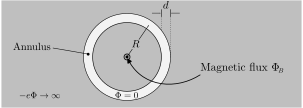
\includegraphics[width=0.4\textwidth]{annulus}
\end{figure}

Now, suppose we thread magnetic flux (e.g., using a solenoid) through
the origin, which lies in the region enclosed by the annulus.  This
flux can be described via the vector potential
\begin{equation}
  \mathbf{A}(r,\phi) = \frac{\Phi_B}{2\pi r} \, \hat{e}_\phi.
  \label{Asolenoid}
\end{equation}
We can verify from Eq.~\eqref{Asolenoid} that the total magnetic flux
through any loop of radius $r$ enclosing the origin is $(\Phi_B/2\pi
r)(2\pi r) = \Phi_B$.  The fact that this is independent of $r$
implies that the magnetic flux density is concentrated in an
infintesimal area surrounding the origin, and zero everywhere
else. However, the vector potential $\mathbf{A}$ is nonzero
everywhere.

The time-independent Schr\"odinger equation is
\begin{equation}
  \frac{1}{2m}\left|-i\hbar\nabla+
  \frac{e\Phi_B}{2\pi r} \, \hat{e}_\phi\right|^2 \psi(r,\phi)
  = E\psi(r,\phi),
  \label{ABschrod}
\end{equation}
with the boundary conditions $\psi(R\pm d/2,0) = 0$.  For sufficiently
large $R$, we can guess that the eigenfunctions have the form
\begin{equation}
  \psi(r,\phi) \approx
  \begin{cases}
  \psi_0 \, \cos\left(\frac{\pi}{d}(r-R)\right)\, e^{i k R \phi},
  & r \in [R-d/2, R + d/2] \\
  0 & \textrm{otherwise}.
  \end{cases}
\end{equation}
This has the form of a ``waveguide mode'', posessing a half-wavelength
wave profile in the $r$ direction (so as to vanish at $r = R \pm d/2$)
and traveling along the azimuthal direction with wavenumber $k$.  The
normalization constant $\psi_0$ is unimportant.  We need the
wavefunction to be single-valued under a $2\pi$ variation in the
azimuthal coordinate, so
\begin{equation}
  k \cdot 2\pi R = 2\pi n \;\;\;\Rightarrow \;\;\; k = \frac{n}{R},
  \;\;\;\mathrm{where}\;\; n \in \mathbb{Z}.
\end{equation}
Plugging this into Eq.~\eqref{ABschrod} yields the energy levels
\begin{align}
  E_n &= \frac{1}{2m} \left[
    \left(\frac{n\hbar}{R} + \frac{e\Phi_B}{2\pi R}\right)^2
    + \left(\frac{\pi\hbar}{d}\right)^2 \right] \\
  &= \frac{e^2}{8\pi^2mR^2} \left(\Phi_B + \frac{nh}{e} \right)^2
  + \frac{\pi^2\hbar^2}{2md^2}.
  \label{abcurves}
\end{align}
In the figure below, these energy levels are sketched versus the
magnetic flux $\Phi_B$.  According to Eq.~\eqref{abcurves}, the
energies are described by a set of quadratic curves, translated along
the $\Phi_B$ axis by integer multiples of $h/e$.  Evidently, varying
$\Phi_B$ will shift the eigen-energies in the annulus, despite the
fact that the magnetic field vanishes in the annulus.  This is a
manifestation of the Aharonov-Bohm effect.

\begin{figure}[h]
  \centering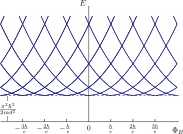
\includegraphics[width=0.65\textwidth]{abring}
\end{figure}

One notable feature of this energy spectrum is that it remains the
same whenever the magnetic flux changes by an exact multiple of $h/e =
4.13567\times10^{-5}\,\mathrm{T}\,\mathrm{m}^2$.  This fundamental
unit of magnetic flux is called the \textbf{magnetic flux quantum}.
Notably, it does not depend on the radius of the annulus, or any other
geometrical parameters of the system.  This is because the invariance
property arises from the gauge symmetry of the Hamiltonian.  When an
extra flux of $nh/e$ (where $n\in\mathbb{Z}$) is threaded through the
annulus, Eq.~\eqref{Asolenoid} tells us that the change in vector
potential is $\Delta \mathbf{A} = (n\hbar/ e r) \hat{e}_\phi$.  We can
undo the effects of this additional vector potential using the gauge
field
\begin{equation}
  \Lambda(r,\phi) = - \frac{n\hbar}{e} \, \phi \;\;\;\Rightarrow
  \begin{cases}\nabla \Lambda &= \displaystyle (n\hbar/er) \hat{e}_\phi
    \\ \displaystyle e^{-ie\Lambda/\hbar} &= \displaystyle e^{in\phi}.
  \end{cases}
\end{equation}
Note that the gauge field $\Lambda$ is not single-valued---but that's
not a problem, since both $\nabla\Lambda$ and the phase factor
$\exp(-ie\Lambda/\hbar)$, which respectively enter into the vector
potential and wavefunction (the ``actual'' physical quantities),
\textit{are} single-valued!

\section{Dirac Theory}

\subsection{The Dirac Hamiltonian}
\label{sec:DiracH}

The $p^2/2m$-type Hamiltonians we have been using describe
non-relativistic particles.  In 1928, Paul Dirac formulated a
Hamiltonian that can describe particles moving close to the speed of
light, thus successfully combining quantum mechanics with the special
theory of relativity. Another triumph of Dirac's theory is that upon
including electromagnetic scalar and vector potentials, the magnetic
moment of the electron is accurately predicted.

Dirac's theory begins from the time-dependent Schr\"odinger equation.
In the wavefunction representation, this has the form
\begin{equation}
  i\hbar\, \partial_t\, \psi(\mathbf{r},t)
  = \hat{H} \psi(\mathbf{r},t).
  \label{schrod}
\end{equation}
Note that the left side has a first-order time derivative.  On the
right side, the Hamiltonian $\hat{H}$ contains spatial derivatives in
the form of momentum operators.  We know that time and space
derivatives of wavefunctions are related to energy and momentum by
\begin{equation}
    i\hbar\, \partial_t\; \leftrightarrow \;
    E, \qquad
    -i\hbar\, \partial_j \;\leftrightarrow \;
    p_j.
\end{equation}
We also know that the energy and momentum of a relativistic particle
are related by
\begin{equation}
  E^2 = m^2c^4 + \sum_{j=1}^3 p_j^2c^2,
  \label{Erelativistic}
\end{equation}
where $m$ is the rest mass and $c$ is the speed of light.  Note that
$E$ and $p$ appear to the same order in this equation.  (Following the
usual practice in relativity theory, we use Roman indices $j \in
\{1,2,3\}$ for the spatial coordinates $\{x,y,z\}$.)

Since the left side of the Schr\"odinger equation \eqref{schrod} has a
first-order time derivative, a relativistic Hamiltonian should involve
first-order spatial derivatives.  So we make the guess
\begin{equation}
  \hat{H} = \alpha_0 mc^2 + \sum_{j=1}^3 \alpha_j \hat{p}_j c,
  \label{Dirac0}
\end{equation}
where $\hat{p}_j \equiv -i\hbar \partial/\partial x_j$.  The $mc^2$
and $c$ factors are placed for later convenience.  We now need to
determine the ``coefficients'' $\alpha_0$, $\alpha_1$, $\alpha_2$, and
$\alpha_3$, which are dimensionless.

For a wavefunction with definite momentum $\mathbf{p}$ and energy
$E$,
\begin{equation}
  \hat{H}\psi = E \psi \;\;\;\Rightarrow \;\;\;
  \left(\alpha_0mc^2 + \sum_{j=1}^3\alpha_j p_jc\right) \psi = E\,\psi,
\end{equation}
where the $\hat{p}_j$ operators are replaced with definite numbers.
If $\psi$ is a scalar, this would imply $\alpha_0 mc^2 +
\sum_{j}\alpha_j p_j c = E$, which does not match the relativistic
energy-mass-momentum relation \eqref{Erelativistic}.  However, we can
get it to work if the $\alpha$'s are matrices rather than numbers:
\begin{framed}
  \begin{equation}
    \hat{H} = \hat{\alpha}_0 mc^2 + \sum_{j=1}^3 \hat{\alpha}_j \hat{p}_j c,
    \;\; \mathrm{where}\;\; \hat{p}_j \equiv -i\hbar\, \partial_j.
    \label{Dirac}
  \end{equation}
\end{framed}
\vskip -0.15in
\noindent
In that case, applying the Hamiltonian twice gives
\begin{equation}
  \left(\hat{\alpha}_0mc^2 + \sum_{j=1}^3\hat{\alpha}_j p_j c\right)^{\!2}\;
  \psi = E^2\,\psi.
\end{equation}
This can be satisfied if
\begin{equation}
  \left(\hat{\alpha}_0 mc^2 + \sum_{j=1}^3\hat{\alpha}_j p_j c\right)^2
  = E^2\, \hat{I},
\end{equation}
where $\hat{I}$ is the identity matrix.  Expanding the square (and
taking care of the fact that the $\hat{\alpha}_\mu$ matrices need not
commute) yields
\begin{equation}
  \hat{\alpha}_0^2 m^2c^4
  + \sum_j \left(\hat{\alpha}_0 \hat{\alpha}_j + \hat{\alpha}_j \hat{\alpha}_0\right) mc^3 p_j
  + \sum_{jj'} \hat{\alpha}_j \hat{\alpha}_{j'} \, p_j p_{j'} = E^2\hat{I}.
\end{equation}
This reduces to Eq.~\eqref{Erelativistic} if the $\hat{\alpha}_\mu$
matrices satisfy
\begin{align}
  \begin{aligned}
    \hat{\alpha}_\mu^2 &= \hat{I} \;\;\; \textrm{for} \;\;\mu=0,1,2,3,
    \;\;\textrm{and} \\
    \hat{\alpha}_\mu \hat{\alpha}_\nu
    + \hat{\alpha}_\nu \hat{\alpha}_\mu &= 0
    \;\;\; \textrm{for} \;\;\mu \ne \nu.
  \end{aligned}
\end{align}
(We use Greek symbols for indices ranging over the four spacetime
coordinates $\{0,1,2,3\}$.)  The above can be written more concisely
using the anticommutator:
\begin{equation}
  \{\hat{\alpha}_\mu, \hat{\alpha}_\nu\} = 2\delta_{\mu\nu},
  \;\;\; \textrm{for} \;\;\mu,\nu=0,1,2,3,
  \label{Dirac_anticomm}
\end{equation}
Also, we need the $\hat{\alpha}_\mu$ matrices to be Hermitian, so that
$\hat{H}$ is Hermitian.

It turns out that the smallest possible Hermitian matrices that can
satisfy Eq.~\eqref{Dirac_anticomm} are $4\times4$ matrices.  The
choice of matrices (or ``representation'') is not uniquely determined.
One particularly useful choice is called the \textbf{Dirac
  representation}:
\begin{align}
  \begin{aligned}
    \hat{\alpha}_0 &= \begin{bmatrix}
      \hat{I}\, & \hat{0} \\ \hat{0} & -\hat{I}
    \end{bmatrix}, \;\;\;
    \hat{\alpha}_1 = \begin{bmatrix}
      \hat{0} & \hat{\sigma}_1 \\ \hat{\sigma}_1 & \hat{0}
    \end{bmatrix} \\
    \hat{\alpha}_2 &= \begin{bmatrix}
      \hat{0} & \hat{\sigma}_2 \\ \hat{\sigma}_2 & \hat{0}
    \end{bmatrix}, \;\;\;
    \hat{\alpha}_3 = \begin{bmatrix}
      \hat{0} & \hat{\sigma}_3 \\ \hat{\sigma}_3 & \hat{0}
    \end{bmatrix},
  \end{aligned}
  \label{alpha_matrices}
\end{align}
where $\{\hat{\sigma}_{1}, \hat{\sigma}_{2}, \hat{\sigma}_{3}\}$
denote the usual Pauli matrices.  Since the $\hat{\alpha}_\mu$'s are
$4\times4$ matrices, it follows that $\psi(\mathbf{r})$ is a
four-component field, not an ordinary scalar wavefunction.

\subsection{Eigenstates of the Dirac Hamiltonian}

According to Eq.~\eqref{Erelativistic}, the energy eigenvalues of the
Dirac Hamiltonian are
\begin{equation}
  E = \pm \sqrt{m^2c^4 + \sum_{j} p_j^2c^2}.
\end{equation}
This is plotted below:

\begin{center}
  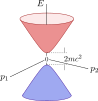
\includegraphics[width=0.27\textwidth]{diraccone}
\end{center}

\noindent
The energy spectrum forms two ``bands''.  For each $\mathbf{p}$, there
are two degenerate positive energy eigenvalues, and two degenerate
negative energy eigenvalues; thus there are four eigenvalues in total,
matching the number of wavefunction components.  The upper band
matches the dispersion relation for a massive relativistic particle,
as desired.  But what about the negative-energy states?  Who ordered
that?

It might be possible for us to ignore the existence of the
negative-energy states, if we are only considering an isolated
electron; we could just declare that the positive-energy states are
the ones we are interested in, and study those.  However, the problem
becomes severe once we let the electron interact with another system,
such as the electromagnetic field.  The positive-energy electron
states then become unstable: due to the availability of
negative-energy states extending down to $E\rightarrow -\infty$, the
electron can repeatedly hop to states with ever more negative energies
by transferring energy to the other system, such as by emitting
photons.  This is obviously problematic.  However, let us wait for a
while (till Section~\ref{sec:positrons}) to discuss how the stability
problem might be resolved.

We will first take some time to analyze the meaning of the Dirac
wavefunction.  The four components represent a four-fold ``internal''
degree of freedom, distinct from the electron's ordinary kinematic
degrees of freedom.  Since there are two energy bands, the assignment
of an electron to the upper or lower band (or some superposition
thereof) consitutes two degrees of freedom.  Each band must then
posssess a two-fold degree of freedom (so that $2\times 2 = 4$), which
turns out to be associated with the electron's spin.

To see explicitly how this works, we must pick a representation for
the $\hat{\alpha}_\mu$ matrices; the choice of representation
determines how the four degrees of freedom are encoded in the
individual wavefunction components.  Let us use the Dirac
representation \eqref{alpha_matrices}.  In this case, it is convenient
to divide the components into upper and lower parts,
\begin{equation}
  \psi(\mathbf{r},t) = \begin{bmatrix}\psi_A(\mathbf{r},t)
    \\ \psi_B(\mathbf{r},t)
  \end{bmatrix},
\end{equation}
where $\psi_A$ and $\psi_B$ have two components each.  Then, for an
eigenstate with energy $E$ and momentum $\mathbf{p}$, applying
\eqref{alpha_matrices} to the Dirac equation \eqref{Dirac} gives
\begin{align}
  \psi_A &= \frac{1}{E - mc^2} \sum_j \hat{\sigma}_j p_j \psi_B,
  \label{dirac_nonrel1} \\
  \psi_B &= \frac{1}{E + mc^2} \sum_j \hat{\sigma}_j p_j \psi_A.
  \label{dirac_nonrel2}
\end{align}
Consider the non-relativistic limit, $|\mathbf{p}| \rightarrow 0$, for
which $E$ approaches either $mc^2$ or $-mc^2$.  For the upper band ($E
\gtrsim mc^2$), the vanishing of the denominator in
Eq.~\eqref{dirac_nonrel1} tells us that the wavefunction is dominated
by $\psi_A$.  Conversely, for the lower band ($E \lesssim -mc^2$),
Eq.~\eqref{dirac_nonrel2} tells us that the wavefunction is dominated
by $\psi_B$.  We can thus associate the upper ($A$) and lower ($B$)
components with the band degree of freedom.  But note that this
association holds only in the non-relativistic limit!  In the
relativistic case, upper-band states can have non-vanishing values in
the $B$ components, and vice versa.

\subsection{Dirac electrons in an electromagnetic field}
\label{sec:diracem}

To continue pursuing our objective of interpreting the Dirac
wavefunction, we must determine how the electron interacts with an
electromagnetic field.  We introduce electromagnetism by following the
same procedure as in the non-relativistic theory
(Section~\ref{sec:nonrel}): add $-e\Phi(\mathbf{r},t)$ as a scalar
potential function, and add the vector potential via the substitution
\begin{equation}
  \hat{\mathbf{p}} \rightarrow \hat{\mathbf{p}}
  + e\mathbf{A}(\hat{\mathbf{r}},t).  
\end{equation}
Applying this recipe to the Dirac Hamiltonian (\ref{Dirac}) yields
\begin{equation}
  i\hbar \, \partial_t \psi
  = \left\{\hat{\alpha}_0 mc^2 -e\Phi(\mathbf{r},t)
  + \sum_{j} \hat{\alpha}_j \Big[-i\hbar\,\partial_j
    +eA_j(\mathbf{r},t) \Big] c\right\}\psi(\mathbf{r},t).
  \label{DiracEM}
\end{equation}
You can check that this has the same gauge symmetry properties as the
non-relativistic theory discussed in Section~\ref{sec:gauge}.

In the Dirac representation \eqref{alpha_matrices},
Eq.~\eqref{DiracEM} reduces to
\begin{align}
  i\hbar\, \partial_t \, \psi_A
  &= \big(+mc^2 -e\Phi \big)\,
  \psi_A
  \,+\, \sum_{j} \hat{\sigma}_j \big(-i\hbar\partial_j
    +eA_j \big) \,c\;\psi_B \label{Dirac2a} \\
  i\hbar\, \partial_t \, \psi_B
  &= \big(- mc^2 -e\Phi\big)\,
  \psi_B \,+\, \sum_{j} \hat{\sigma}_j \big(-i\hbar\partial_j
    +eA_j \big)\, c\;\psi_A, \label{Dirac2b}
\end{align}
where $\psi_A$ and $\psi_B$ are the previously-introduced
two-component objects corresponding to the upper and lower halves of
the Dirac wavefunction.

In the non-relativistic limit, solutions to the above equations can be
cast in the form
\begin{align}
  \begin{aligned}
  \psi_{A}(\mathbf{r},t) &= \Psi_{A}(\mathbf{r},t)\,
  \exp\left[-i\left(\frac{mc^2}{\hbar}\right)t\right] \\
  \psi_{B}(\mathbf{r},t) &= \Psi_{B}(\mathbf{r},t)\,
  \exp\left[-i\left(\frac{mc^2}{\hbar}\right)t\right].
  \end{aligned}
\end{align}
The exponentials on the right side are the $\exp(-i\omega t)$ factor
corresponding to the rest energy $mc^2$, which dominates the
electron's energy in the non-relativistic limit.  (Note that by using
$+mc^2$ rather than $-mc^2$, we are explicitly referencing the
positive-energy band.)  If the electron is in an eigenstate with
$\mathbf{p} = 0$ and there are no electromagnetic fields, $\Psi_A$ and
$\Psi_B$ would just be constants.  Now suppose the electron is
non-relativistic but not in a $\mathbf{p} = 0$ eigenstate, and the
electromagnetic fields are weak but not necessarily vanishing.  In
that case, $\Psi_A$ and $\Psi_B$ are functions that vary with $t$, but
slowly.

Plugging this ansatz into Eqs.~\eqref{Dirac2a}--\eqref{Dirac2b} gives
\begin{align}
  i\hbar\, \partial_t \, \Psi_A
  &= -e\Phi\; \Psi_A
  \,+\, \sum_{j} \hat{\sigma}_j \big(-i\hbar\partial_j
    +eA_j \big) c\;\Psi_B \label{Dirac3a} \\
  \big(i\hbar\, \partial_t \, + 2mc^2 + e\Phi\big)
  \Psi_B
  &= \sum_{j} \hat{\sigma}_j \big(-i\hbar\partial_j
    +eA_j \big) c\;\Psi_A. \label{Dirac3b}
\end{align}
On the left side of Eq.~\eqref{Dirac3b}, the $2mc^2$ term dominates
over the other two, so
\begin{equation}
  \Psi_B \;\approx\; \frac{1}{2mc}\, \sum_{j}
  \hat{\sigma}_j \big(-i\hbar\partial_j +eA_j \big) \;\Psi_A.
\end{equation}
Plugging this into Eq.~\eqref{Dirac3a} yields
\begin{equation}
  i\hbar\, \partial_t \, \Psi_A
  = \left\{-e\Phi \,+\, \frac{1}{2m} \sum_{jk} \hat{\sigma}_j \hat{\sigma}_k
  \big(-i\hbar\partial_j +eA_j \big)
  \big(-i\hbar\partial_k +eA_k \big) \right\}\;\Psi_A.
\end{equation}
Using the identity $\hat{\sigma}_j\hat{\sigma}_k = \delta_{jk}\hat{I}
+ i \sum_i \varepsilon_{ijk}\sigma_i$:
\begin{align}
  \begin{aligned}
  i\hbar\, \partial_t \, \Psi_A
  &= \Bigg\{-e\Phi
  \,+\, \frac{1}{2m} \big|-i\hbar\nabla +e\mathbf{A} \big|^2 \\
  &\qquad+\, \frac{i}{2m} \sum_{ijk} \varepsilon_{ijk} \hat{\sigma}_i
  \big(-i\hbar\partial_j +eA_j \big)
  \big(-i\hbar\partial_k +eA_k \big)
  \Bigg\} \Psi_A.
  \end{aligned}
\end{align}
Look carefully at the last term in the curly brackets.  Expanding the
square yields
\begin{equation*}
  \frac{i}{2m}\sum_{ijk}\varepsilon_{ijk}\hat{\sigma}_i
  \Big(-\partial_j\partial_k -i\hbar e \partial_jA_k
  - i\hbar e \big[A_k\partial_j + A_j\partial_k \big]
  + e^2A_jA_k \Big).
\end{equation*}
Due to the antisymmetry of $\varepsilon_{ijk}$, all terms inside the
parentheses that are symmetric under $j$ and $k$ cancel out when
summed over.  The only survivor is the second term, which gives
\begin{equation}
  \frac{\hbar e}{2m}\sum_{ijk}\varepsilon_{ijk}\hat{\sigma}_i
  \partial_jA_k = \frac{\hbar e}{2m} \hat{\boldsymbol{\sigma}}
  \,\cdot\, \mathbf{B}(\mathbf{r},t),
\end{equation}
where $\mathbf{B} = \nabla\times\mathbf{A}$ is the magnetic field.
Hence,
\begin{equation}
  i\hbar\, \partial_t \, \Psi_A
  = \left\{-e\Phi
  \,+\, \frac{1}{2m} \big|-i\hbar\nabla +e\mathbf{A} \big|^2
  \,-\, \left(-\frac{\hbar e}{2m}\, \hat{\boldsymbol{\sigma}}\right)
  \,\cdot\, \mathbf{B} \right\} \Psi_A.
\end{equation}
This is an exact match for Eq.~\eqref{quantumH}, except that the
Hamiltonian has an additional term of the form $-
\hat{\boldsymbol{\mu}} \cdot \hat{\mathbf{B}}$.  This additional term
corresponds to the potential energy of a magnetic dipole of moment
$\boldsymbol{\mu}$ in a magnetic field $\mathbf{B}$.  The Dirac theory
therefore predicts the electron's magnetic dipole moment to be
\begin{equation}
  |\boldsymbol{\mu}| = \frac{\hbar e}{2m}.
  \label{Diracmu}
\end{equation}
Remarkably, this matches the experimentally-observed magnetic dipole
moment to about one part in $10^3$.  We thus see that the electron's
magnetic dipole moment is not an arbitrary quantity, but an outcome of
combining quantum mechanics with relativity.  The residual mismatch
between Eq.~\eqref{Diracmu} and the actual magnetic dipole moment of
the electron is understood to arise from quantum fluctuations of the
electronic and electromagnetic quantum fields; this ``anomalous
magnetic moment'' can be calculated using the full theory of quantum
electrodynamics, and matches experiment to around one part in $10^9$,
making it one of the most precise theoretical predictions in physics.
For details, see \hyperref[cite:zee]{Zee (2010)}.

It is also noteworthy that we did not set out to include spin in the
theory, yet it arose, seemingly unavoidably, as a by-product of
formulating a relativistic theory of the electron.  This is a
manifestation of the fact that relativistic quantum theory is more
constrained than non-relativistic quantum theory.  Relativistic
symmetries demand that spin cannot be an optional part of the theory,
but must be fully accounted for.

\subsection{Positrons and Dirac Field Theory}
\label{sec:positrons}

To stabilize the electron against decay into negative-energy states,
Dirac suggested that what we regard as the ``vacuum'' may actually be
a state, called the \textbf{Dirac sea}, in which all the
negative-energy states are occupied.  Then the Pauli exclusion
principle would prevent decay into the negative-energy states.

At first blush, the idea seems ridiculous; how can the vacuum contain
an infinite number of particles?  However, we shall see that the idea
is more plausible if we re-interpret the Dirac theory as a
single-particle \textit{construction} which arises from a more
fundamental quantum field theory.  The Dirac sea idea is an inherently
multi-particle concept, and we saw in Chapter 3 that quantum field
theory is a natural framework for describing multi-particle quantum
states.  Let us therefore develop this quantum field theory.

Consider again the eigenstates of the single-particle Dirac
Hamiltonian with definite momenta and energies.  Denote the
positive-energy wavefunctions by
\begin{equation}
  \frac{u_{\mathbf{k}\sigma} \, e^{i\mathbf{k}\cdot \mathbf{r}}}{(2\pi)^{3/2}}
  = \langle \mathbf{r} | \mathbf{k}, +, \sigma\rangle,
  \quad\mathrm{where}\;\;
  \hat{H} |\mathbf{k}, +, \sigma\rangle
  = \epsilon_{\mathbf{k}\sigma} |\mathbf{k}, +, \sigma\rangle.
  \label{Diraces1}
\end{equation}
The negative-energy wavefunctions are
\begin{equation}
  \frac{v_{\mathbf{k}\sigma} \, e^{-i\mathbf{k}\cdot \mathbf{r}}}{(2\pi)^{3/2}}
  = \langle \mathbf{r} | \mathbf{k}, -, \sigma\rangle,
  \quad\mathrm{where}\;\;
  \hat{H} |\mathbf{k}, -, \sigma\rangle
  = - \epsilon_{\mathbf{k}\sigma} |\mathbf{k}, -, \sigma\rangle.
  \label{Diraces2}
\end{equation}
Note that $|\mathbf{k}, -, \sigma\rangle$ denotes a negative-energy
eigenstate with momentum $-\hbar\mathbf{k}$, not $\hbar\mathbf{k}$.
The reason for this notation, which uses different symbols to label
the positive-energy and negative-energy states, will become clear
later.  Each of the $u_{\mathbf{k}\sigma}$ and $v_{\mathbf{k}\sigma}$
terms are four-component objects (spinors), and for any given
$\mathbf{k}$, the set
\begin{equation*}
  \{ u_{\mathbf{k}\sigma}, v_{\mathbf{k},\sigma}\;\;  | \;\; \sigma = 1,2  \}
\end{equation*}
forms an orthonormal basis for the four-dimensional spinor space.
Thus,
\begin{equation}
  \sum_{n} \left(u^n_{\mathbf{k}\sigma}\right)^* u^n_{\mathbf{k}\sigma'} = \delta_{\sigma\sigma'}, \;\;
  \sum_{n} \left(u^n_{\mathbf{k}\sigma}\right)^* v^n_{\mathbf{k}\sigma'} = 0, \;\;
  \textrm{etc.}
  \label{uvorthog}
\end{equation}
Here we use the notation where $u^n_{\mathbf{k}\sigma}$ is the $n$-th
component of the $u_{\mathbf{k}\sigma}$ spinor, etc.

We now follow the second quantization procedure from Chapter 3.  We
introduce a (fermionic) Fock space $\mathscr{H}_F$, as well as a set
of creation/annihilation operators:
\begin{align*}
  \hat{b}_{\mathbf{k}\sigma}^\dagger \;\; \mathrm{and} \;\; \hat{b}_{\mathbf{k}\sigma}
  &\;\;\mathrm{create/annihilate} \;\; |\mathbf{k}, +, \sigma\rangle\\
  \hat{d}_{\mathbf{k}\sigma}^\dagger \;\; \mathrm{and} \;\; \hat{d}_{\mathbf{k}\sigma}
  &\;\;\mathrm{create/annihilate} \;\; |\mathbf{k}, -, \sigma\rangle.
\end{align*}
These obey the fermionic anticommutation relations
\begin{align}
  \begin{aligned}
    \{\hat{b}_{\mathbf{k}\sigma}, \hat{b}_{\mathbf{k}'\sigma'}^\dagger \}
    = \delta^3(\mathbf{k}-\mathbf{k}') \, \delta_{\sigma\sigma'}, \quad
    \{\hat{d}_{\mathbf{k}\sigma}, \hat{d}_{\mathbf{k}'\sigma'}^\dagger \}
    = \delta^3(\mathbf{k}-\mathbf{k}') \, \delta_{\sigma\sigma'} \\
    \{\hat{b}_{\mathbf{k}\sigma}, \hat{b}_{\mathbf{k}'\sigma'} \} = 
    \{\hat{b}_{\mathbf{k}\sigma}, \hat{d}_{\mathbf{k}'\sigma'} \} = 
    \{\hat{d}_{\mathbf{k}\sigma}, \hat{d}_{\mathbf{k}'\sigma'} \} = 0, \;\;\textrm{etc.}
  \end{aligned}
  \label{Diracanticommutation0}
\end{align}
The Hamiltonian is
\begin{equation}
  \hat{H} = \int d^3k \sum_\sigma \epsilon_{\mathbf{k}\sigma} \left(
  \hat{b}^\dagger_{\mathbf{k}\sigma} \hat{b}_{\mathbf{k}\sigma}
  - \hat{d}^\dagger_{\mathbf{k}\sigma} \hat{d}_{\mathbf{k}\sigma}
  \right),
  \label{HDiracQFT0}
\end{equation}
and applying the annihilation operators to the vacuum state
$|\varnothing\rangle$ gives zero:
\begin{equation}
  \hat{b}_{\mathbf{k}\sigma} |\varnothing\rangle =
  \hat{d}_{\mathbf{k}\sigma} |\varnothing\rangle = 0.
\end{equation}

When formulating bosonic field theory, we defined a local field
annihilation operator that annihilates a particle at a given point
$\mathbf{r}$.  In the infinite-system limit, this took the form
\begin{equation}
  \hat{\psi}(\mathbf{r})
  = \int d^3k \; \varphi_{\mathbf{k}}(\mathbf{r}) \, \hat{a}_{\mathbf{k}},
\end{equation}
and the orthonormality of the $\varphi_{\mathbf{k}}$ wavefunctions
implied that $[\hat{\psi}(\mathbf{r}),
  \hat{\psi}^\dagger(\mathbf{r}')] =
\delta^3(\mathbf{r}-\mathbf{r}')$.  Similarly, we can use the Dirac
Hamiltonian's eigenfunctions \eqref{Diraces1}--\eqref{Diraces2} to
define
\begin{equation}
  \hat{\psi}_n(\mathbf{r})
  = \int \frac{d^3k}{(2\pi)^{3/2}} \; \sum_\sigma
  \left(
  u^n_{\mathbf{k}\sigma} e^{i\mathbf{k}\cdot\mathbf{r}} \, \hat{b}_{\mathbf{k}\sigma}
  + v^n_{\mathbf{k}\sigma} e^{-i\mathbf{k}\cdot\mathbf{r}} \, \hat{d}_{\mathbf{k}\sigma}\right).
  \label{Diracpsi0}
\end{equation}
Note that the two terms in the parentheses arise simply because the
positive-energy and negative-energy states are denoted by
differently-labeled annihilation operators.  Moreover, since the
wavefunctions are four-component spinors, the field operators have an
explicit spinor index $n$.  Using the spinor orthonormality conditions
\eqref{uvorthog} and the anticommutation relations
\eqref{Diracanticommutation0}, we can show that
\begin{equation}
  \left\{\hat{\psi}_n(\mathbf{r}), \hat{\psi}_{n'}^{\dagger}(\mathbf{r}')\right\}
  = \delta_{nn'}\, \delta^3(\mathbf{r}-\mathbf{r}'),
\end{equation}
with all other anticommutators vanishing.  Hence,
$\hat{\psi}_n(\mathbf{r})$ can be regarded as an operator that
annihilates a four-component fermion at point $\mathbf{r}$.

Now let us \textit{define} the operators
\begin{equation}
  \hat{c}_{\mathbf{k}\sigma} = \hat{d}^\dagger_{\mathbf{k}\sigma}.
\end{equation}
Then the fermionic anticommutation relations can be re-written as
\begin{align}
  \begin{aligned}
    \{\hat{b}_{\mathbf{k}\sigma}, \hat{b}_{\mathbf{k}'\sigma'}^\dagger \}
    = \delta^3(\mathbf{k}-\mathbf{k}') \, \delta_{\sigma\sigma'}, \quad
    \{\hat{c}_{\mathbf{k}\sigma}, \hat{c}_{\mathbf{k}'\sigma'}^\dagger \}
    = \delta^3(\mathbf{k}-\mathbf{k}') \, \delta_{\sigma\sigma'} \\
    \{\hat{b}_{\mathbf{k}\sigma}, \hat{b}_{\mathbf{k}'\sigma'} \} = 
    \{\hat{b}_{\mathbf{k}\sigma}, \hat{c}_{\mathbf{k}'\sigma'} \} = 
    \{\hat{c}_{\mathbf{k}\sigma}, \hat{c}_{\mathbf{k}'\sigma'} \} = 0, \;\;\textrm{etc.}
  \end{aligned}
  \label{Diracanticommutators}
\end{align}
This means that $\hat{c}^\dagger_{\mathbf{k}\sigma}$ and
$\hat{c}_{\mathbf{k}\sigma}$ formally satisfy the criteria to be
regarded as creation and annihilation operators.  The particle created
by $\hat{c}^\dagger_{\mathbf{k}\sigma}$ is called a \textbf{positron},
and is equivalent to the \textit{absence} of a $d$-type particle
(i.e., a negative-energy electron).

The Hamiltonian \eqref{HDiracQFT0} can now be written as
\begin{equation}
  \hat{H} = \int d^3k \sum_\sigma \epsilon_{\mathbf{k}\sigma} \left(
  \hat{b}^\dagger_{\mathbf{k}\sigma} \hat{b}_{\mathbf{k}\sigma}
  + \hat{c}^\dagger_{\mathbf{k}\sigma} \hat{c}_{\mathbf{k}\sigma}
  \right) \;\; + \;\; \textrm{constant},
  \label{HDiracQFT}
\end{equation}
which explicitly shows that the positrons have positive energies
(i.e., the absence of a negative-energy particle is equivalent to the
presence of a positive-energy particle).  With further analysis, which
we will skip, it can be shown that the positron created by
$\hat{c}^\dagger_{\mathbf{k}\sigma}$ has positive charge $e$ and
momentum $\hbar\mathbf{k}$.  The latter is thanks to the definition
adopted in Eq.~\eqref{Diraces2}; the absence of a momentum $-\hbar
\mathbf{k}$ particle is equivalent to the presence of a momentum
$\hbar \mathbf{k}$ particle.  As for the field annihilation operator
\eqref{Diracpsi0}, it can be written as
\begin{equation}
  \hat{\psi}_n(\mathbf{r})
  = \int \frac{d^3k}{(2\pi)^{3/2}} \; \sum_\sigma
  \left(
  u^n_{\mathbf{k}\sigma} e^{i\mathbf{k}\cdot\mathbf{r}} \, \hat{b}_{\mathbf{k}\sigma}
  + v^n_{\mathbf{k}\sigma} e^{-i\mathbf{k}\cdot\mathbf{r}} \,
  \hat{c}^\dagger_{\mathbf{k}\sigma}\right).
  \label{Diracpsi}
\end{equation}

The $c$-type annihilation operators do \textit{not} annihilate
$|\varnothing\rangle$.  However, let us define
\begin{equation}
  |\varnothing'\rangle = \prod_{\mathbf{k}\sigma} \hat{d}_{\mathbf{k}\sigma}^\dagger
  |\varnothing\rangle,
\end{equation}
which is evidently a formal description of the Dirac sea state.  Then
\begin{equation}
  \hat{c}_{\mathbf{k}\sigma} |\varnothing'\rangle = 
  \hat{c}^\dagger_{\mathbf{k}\sigma} \prod_{\mathbf{k}'\sigma'}
  \hat{d}_{\mathbf{k}'\sigma'}^\dagger |\varnothing\rangle = 0.
\end{equation}

Having done all this, we can regard the quantum field theory as being
defined in terms of $b$-type and $c$-type operators, using the
anticommutators \eqref{Diracanticommutators}, the Hamiltonian
\eqref{HDiracQFT}, and the field operator \eqref{Diracpsi}, along with
the vacuum state $|\varnothing'\rangle$.  The elementary particles are
electrons and positrons, which have strictly positive energies.  Then
the whole single-particle Dirac theory, with its quirky
negative-energy states, can be interpreted as a special construct that
allows us to map the quantum field theory into single-particle
language.  It is the quantum field theory, however, that is more
fundamental.

There is much more to understand about the structure and
interpretation of the Dirac single-particle theory and quantum field
theory, which we will not pursue here.  One particularly important
issue involves how the particles, and the underlying quantum field,
transform under Lorentz boosts and other changes in coordinate system.
For these details, the reader is referred to
\hyperref[cite:dyson]{Dyson (1951)}.

\section{Quantizing the electromagnetic field}
\label{sec:em_quantization}

We have previously seen how to quantize a simple scalar boson field
(Chapter 3, Sec.~V.C): the classical field is decomposed into normal
modes, and each mode is quantized by treating it as an independent
oscillator, with its own creation and annihilation operators.  By
comparing the oscillator energies in the classical and quantum
regimes, we derive the Hermitian operator corresponding to the
classical field variable, expressed in terms of the creation and
annihilation operators.

We will use this approach, with minor adjustments, to quantize the
electromagnetic field.

First, consider a ``source-free'' electromagnetic field---i.e., with
no electric charges and currents.  Without sources, Maxwell's
equations (in SI units, and in a vacuum) reduce to:
\begin{align}
  \nabla\cdot \mathbf{E} &= 0 \label{max1} \\
  \nabla\cdot \mathbf{B} &= 0 \label{max2}\\
  \nabla\times \mathbf{E} &= -\frac{\partial \mathbf{B}}{\partial t} \label{max3}\\
  \nabla\times \mathbf{B} &= \frac{1}{c^2} \frac{\partial \mathbf{E}}{\partial t}.
  \label{max4}
\end{align}
Once again, we introduce the scalar potential $\Phi$ and vector
potential $\mathbf{A}$:
\begin{align}
  \mathbf{E} &= - \nabla \Phi - \frac{\partial\mathbf{A}}{\partial t} \\
  \mathbf{B} &= \nabla \times \mathbf{A}.
\end{align}
These relations cause Eqs.~\eqref{max2} and \eqref{max3} to be
satisfied automatically, via vector identities.  The other two Maxwell
equations, \eqref{max1} and \eqref{max4}, become:
\begin{align}
  \nabla^2 \Phi &= -\frac{\partial}{\partial t} \nabla \cdot \mathbf{A} \label{max5} \\
  \left(\nabla^2 - \frac{1}{c^2}\frac{\partial^2}{\partial t^2}\right)
  \mathbf{A} &= \nabla\left[\frac{1}{c^2}\frac{\partial}{\partial t}  \Phi + \nabla\cdot\mathbf{A}\right]. \label{max6}
\end{align}

In the next step, we choose a convenient gauge called the
\textbf{Coulomb gauge}:
\begin{equation}
  \Phi = 0, \;\;\; \nabla \cdot \mathbf{A} = 0.
  \label{coulomb}
\end{equation}
(To see that we can always make such a gauge choice, suppose we start
out with a scalar potential $\Phi_0$ and vector potential
$\mathbf{A}_0$ not satisfying \eqref{coulomb}.  Perform a gauge
transformation with a gauge field $\Lambda(\mathbf{r}, t) = - \int^t
dt'\; \Phi_0(\mathbf{r}, t')$.  Then the new scalar potential is $\Phi
= \Phi_0 + \dot{\Lambda} = 0$; moreover, the new vector potential
satisfies
\begin{equation}
  \nabla\cdot\mathbf{A} = \nabla\cdot \mathbf{A}_0 - \nabla^2 \Lambda
  = \nabla\cdot \mathbf{A}_0 + \int^t dt'\; \nabla^2\Phi_0(\mathbf{r}, t').
\end{equation}
Upon using Eq.~\eqref{max5}, we find that $\nabla\cdot\mathbf{A} =
0$.)

In the Coulomb gauge, Eq.~\eqref{max5} is automatically satisfied.
The remaining equation, \eqref{max6}, simplifies to
\begin{equation}
  \left(\nabla^2 - \frac{1}{c^2}\frac{\partial^2}{\partial t^2}\right)
  \mathbf{A} = 0. \label{max8}
\end{equation}
Hence, we deduce that the normal modes are \textbf{light waves} that
have the plane-wave form
\begin{equation}
  \mathbf{A}(\mathbf{r},t) = \Big(\mathcal{A}\,
  \, e^{i(\mathbf{k}\cdot\mathbf{r} - \omega t)} + \mathrm{c.c.}\Big)\, \hat{e},
  \label{lightplanewave}
\end{equation}
where $\mathcal{A}$ is a complex number (the \textbf{mode amplitude})
that specifies the magnitude and phase of the plane wave, $\hat{e}$ is
a real unit vector (the \textbf{polarization vector}) that specifies
which direction the vector potential points along, and
``c.c.''~denotes the complex conjugate of the first term.  Referring
to Eq.~\eqref{max8}, we see that the frequency $\omega$ must satisfy
\begin{equation}
  \omega = c|\mathbf{k}|.
\end{equation}
For convenience, suppose for now that we put the electromagnetic field
in a box of volume $V = L^3$, with periodic boundary conditions, so
that the $\mathbf{k}$ vectors form a discrete set:
\begin{equation}
  k_j = \frac{2\pi n_j}{L}, \;\; n_j \in \mathbf{Z}, \;\;\mathrm{for}
  \;\; j = 1,2,3.
\end{equation}
We will take the $L \rightarrow \infty$ limit at the very end.

Since $\nabla \cdot \mathbf{A} = 0$, it must also be the case that
\begin{equation}
  \mathbf{k} \cdot \hat{e} = 0.
\end{equation}
In other words, the polarization vector is perpendicular to the
propagation direction.  For each $\mathbf{k}$, there are two
orthogonal polarization, which can be labelled by an index $\lambda =
1,2$.

Hence, the vector potential field can be generally decomposed into a
discrete superposition of plane waves:
\begin{equation}
  \mathbf{A}(\mathbf{r},t) = \sum_{\mathbf{k}\lambda} 
  \Big(\mathcal{A}_{\mathbf{k}\lambda} \, e^{i(\mathbf{k}\cdot\mathbf{r} - \omega_{\mathbf{k}} t)}
  + \mathrm{c.c.}\Big)\, \hat{e}_{\mathbf{k}\lambda},
  \;\;\; \mathrm{where}
  \;\;\;\omega_{\mathbf{k}} = c|\mathbf{k}|.
\end{equation}
To convert the classical field theory into a quantum field theory, for
each $(\mathbf{k},\lambda)$ we define an independent set of creation
and annihilation operators:
\begin{equation}
  \big[\hat{a}_{\mathbf{k}\lambda}, \hat{a}_{\mathbf{k}'\lambda'}^\dagger\big]
  = \delta_{\mathbf{k}\mathbf{k}'} \delta_{\lambda\lambda'}, \;\;\;
  \big[\hat{a}_{\mathbf{k}\lambda}, \hat{a}_{\mathbf{k}'\lambda'}\big]
  = \big[\hat{a}_{\mathbf{k}\lambda}^\dagger, \hat{a}_{\mathbf{k}'\lambda'}^\dagger\big]
  = 0.
\end{equation}
Then the Hamiltonian for the electromagnetic field is
\begin{equation}
  \hat{H} = \sum_{\mathbf{k}\lambda} \hbar \omega_{\mathbf{k}} \,
  \hat{a}^\dagger_{\mathbf{k}\lambda} \hat{a}_{\mathbf{k}\lambda},
  \;\;\; \mathrm{where}
  \;\;\;\omega_{\mathbf{k}} = c|\mathbf{k}|.
\end{equation}
And the vector potential is promoted into a Hermitian operator in the
Heisenberg picture:
\begin{equation}
  \hat{\mathbf{A}}(\mathbf{r},t) = \sum_{\mathbf{k}\lambda} 
  \mathcal{C}_{\mathbf{k}\lambda}\,
  \Big(\hat{a}_{\mathbf{k}\lambda} \, e^{i(\mathbf{k}\cdot\mathbf{r} - \omega_{\mathbf{k}} t)}
  + \mathrm{h.c.}\Big)\, \hat{e}_{\mathbf{k}\lambda}.
\end{equation}
Here, $\mathcal{C}_{\mathbf{k}\lambda}$ is a constant to be
determined, and ``h.c.''~denotes the Hermitian conjugate.  The
creation and annihilation operators in this equation are Schr\"odinger
picture ($t = 0$) operators (see Chapter 3, Sec.~V.C).  The particles
that they create/annihilate are called \textbf{photons}---elementary
particles of light.

To find $\mathcal{C}_{\mathbf{k}\lambda}$, we compare the quantum and
classical energies.  Consider the quantum case first: suppose the
electromagnetic field is in a coherent state
$|\alpha_{\mathbf{k}\lambda}\rangle$ such that
\begin{equation}
  \hat{a}_{\mathbf{k}\lambda}|\alpha_{\mathbf{k}\lambda}\rangle
  = \alpha_{\mathbf{k}\lambda}|\alpha_{\mathbf{k}\lambda}\rangle,
  \label{coherent}
\end{equation}
for some $\alpha_{\mathbf{k}\lambda} \in \mathbb{C}$.  Then the mean
squared expectation value of $A^2$, where $A$ is the vector potential
component parallel to the polarization vector
$\hat{e}_{\mathbf{k}\lambda}$, is
\begin{equation}
  \overline{\langle \alpha_{\mathbf{k}\lambda} | \hat{A}^2(\mathbf{r},t) | \alpha_{\mathbf{k}\lambda}\rangle}
  = 2 \, |\mathcal{C}_{\mathbf{k}\lambda}|^2 \, |\alpha_{\mathbf{k}\lambda}|^2.
  \label{quant_Asq}
\end{equation}
The energy is
\begin{equation}
  E = \hbar\omega_{\mathbf{k}} |\alpha_{\mathbf{k}\lambda}|^2.
  \label{quant_energy}
\end{equation}

Now compare this to the classical case.  The energy density (energy
per unit volume) of a classical source-free electromagnetic plane wave
is
\begin{equation}
  \overline{u} = \varepsilon_0\, \omega^2 \, \overline{A^2},
\end{equation}
where $\varepsilon_0$ is the permittivity of free space.  Combining
this with Eqs.~\eqref{quant_Asq} and \eqref{quant_energy}, and taking
$E = \overline{u} V$, yields
\begin{align}
  \hbar\omega_{\mathbf{k}} |\alpha_{\mathbf{k}\lambda}|^2 &=
  \left(\varepsilon_0\, \omega^2\right) \,
  \left(2 \, |\mathcal{C}_{\mathbf{k}\lambda}|^2 \, |\alpha_{\mathbf{k}\lambda}|^2\right)\, V \\
  \Rightarrow \quad \mathcal{C}_{\mathbf{k}\lambda} &= \sqrt{\frac{\hbar}{2\varepsilon_0\omega_{\mathbf{k}}V}}.
\end{align}
We thus arrive at the result
\begin{align}
\boxed{\qquad
  \begin{aligned}
    \hat{H} &= \sum_{\mathbf{k}\lambda} \hbar \omega_{\mathbf{k}} \,
    \hat{a}^\dagger_{\mathbf{k}\lambda} \hat{a}_{\mathbf{k}\lambda} \\
  \hat{\mathbf{A}}(\mathbf{r},t) &= \sum_{\mathbf{k}\lambda} 
  \sqrt{\frac{\hbar}{2\varepsilon_0\omega_{\mathbf{k}}V}}\,
  \Big(\hat{a}_{\mathbf{k}\lambda} \, e^{i(\mathbf{k}\cdot\mathbf{r} - \omega_{\mathbf{k}} t)}
  + \mathrm{h.c.}\Big)\, \hat{e}_{\mathbf{k}\lambda} \\
  \omega_{\mathbf{k}} &= c|\mathbf{k}|,  \;\;\;
  \big[\hat{a}_{\mathbf{k}\lambda}, \hat{a}_{\mathbf{k}'\lambda'}^\dagger\big]
  = \delta_{\mathbf{k}\mathbf{k}'} \delta_{\lambda\lambda'}, \;\;\;
  \big[\hat{a}_{\mathbf{k}\lambda}, \hat{a}_{\mathbf{k}'\lambda'}\big]
  = 0.
  \end{aligned}
  \qquad}
  \label{qed1}
\end{align}
To describe infinite free space rather than a finite-volume box, we
take the $L\rightarrow \infty$ limit and re-normalize the creation and
annihilation operators by the replacement
\begin{equation}
  \hat{a}_{\mathbf{k}\lambda} \rightarrow \sqrt{\frac{(2\pi)^3}{V}} \;
  \hat{a}_{\mathbf{k}\lambda}.
\end{equation}
Then the sums over $\mathbf{k}$ become integrals over the infinite
three-dimensional space:
\begin{align}
\boxed{\qquad
  \begin{aligned}
    \hat{H} &= \int d^3k\sum_{\lambda} \hbar \omega_{\mathbf{k}} \,
    \hat{a}^\dagger_{\mathbf{k}\lambda} \hat{a}_{\mathbf{k}\lambda} \\
  \hat{\mathbf{A}}(\mathbf{r},t) &= \int d^3k \sum_{\lambda} 
  \sqrt{\frac{\hbar}{16\pi^3\varepsilon_0\omega_{\mathbf{k}}}}\,
  \Big(\hat{a}_{\mathbf{k}\lambda} \, e^{i(\mathbf{k}\cdot\mathbf{r} - \omega_{\mathbf{k}} t)}
  + \mathrm{h.c.}\Big)\, \hat{e}_{\mathbf{k}\lambda} \\
  \omega_{\mathbf{k}} &= c|\mathbf{k}|,  \;\;\;
  \big[\hat{a}_{\mathbf{k}\lambda}, \hat{a}_{\mathbf{k}'\lambda'}^\dagger\big]
  = \delta^3(\mathbf{k}-\mathbf{k}') \delta_{\lambda\lambda'}, \;\;\;
  \big[\hat{a}_{\mathbf{k}\lambda}, \hat{a}_{\mathbf{k}'\lambda'}\big]
  = 0.
  \end{aligned}
  \qquad}
  \label{qed2}
\end{align}

\section{The electron-photon interaction}

Now that we have separate quantum theories for the electron and the
electromagnetic field, we can put them together into a theory of
\textbf{quantum electrodynamics}.  This theory will be able to
describe processes involving electrons interacting with the
electromagnetic field by absorbing and/or radiating photons.

In concrete terms, let $\mathscr{H}_{\mathrm{e}}$ denote the Hilbert
space for one electron (for now, we'll use a single-particle rather
than field-theoretical description for the electron).  Let
$\mathscr{H}_{\mathrm{EM}}$ denote the Hilbert space for the
electromagnetic field (i.e., a Fock space for photons).  The states of
the combined system lie in the product space
\begin{equation*}
  \mathscr{H}_e \otimes \mathscr{H}_{\mathrm{EM}}.
\end{equation*}
We seek a Hamiltonian of the form
\begin{equation}
  H = H_e + H_{\mathrm{EM}} + H_{\mathrm{int}},
\end{equation}
where $H_e$ is the Hamiltonian for the ``bare'' electron (either an
ordinary $p^2/2m$-type Hamiltonian, or the Dirac Hamiltonian described
in Section~\ref{sec:DiracH}); $H_{\mathrm{EM}}$ is the Hamiltonian for
the source-free electromagnetic field (derived in
Section~\ref{sec:em_quantization}); and $H_{\mathrm{int}}$ is an
\textbf{interaction Hamiltonian} describing how the electron interacts
with photons.

We can use the discussion in the previous sections as a guide to
finding $H_{\mathrm{int}}$.  Let us once again adopt the Coulomb
gauge, so that the scalar potential is zero, and the electromagnetic
field is solely described via the vector potential.  In
Section~\ref{sec:nonrel}, we saw that the effect of the vector
potential on a charged particle can be described via the substitution
\begin{equation}
  \hat{\mathbf{p}} \rightarrow \hat{\mathbf{p}} +
  e\mathbf{A}(\hat{\mathbf{r}},t).
\end{equation}
In Section~\ref{sec:diracem}, we saw that this substitution is
applicable not just to non-relativistic particles, but also to fully
relativistic particles described by the Dirac Hamiltonian.
Previously, we have treated the $\mathbf{A}$ in this substitution as a
classical object lacking quantum dynamics of its own.  Now, we replace
it by the vector potential \textit{operator} derived in
Section~\ref{sec:em_quantization}:
\begin{equation}
  \hat{\mathbf{A}}(\hat{\mathbf{r}},t) =
  \begin{cases}
    \displaystyle
    \sum_{\mathbf{k}\lambda} 
  \sqrt{\frac{\hbar}{2\varepsilon_0\omega_{\mathbf{k}}V}}\,
  \Big(\hat{a}_{\mathbf{k}\lambda} \, e^{i(\mathbf{k}\cdot\mathbf{r} - \omega_{\mathbf{k}} t)}
  + \mathrm{h.c.}\Big)\, \hat{e}_{\mathbf{k}\lambda}, & (\mathrm{finite}\;\mathrm{volume}) \\
  \displaystyle \int d^3k \sum_{\lambda} 
  \sqrt{\frac{\hbar}{16\pi^3\varepsilon_0\omega_{\mathbf{k}}}}\,
  \Big(\hat{a}_{\mathbf{k}\lambda} \, e^{i(\mathbf{k}\cdot\hat{\mathbf{r}} - \omega_{\mathbf{k}} t)}
  + \mathrm{h.c.}\Big)\, \hat{e}_{\mathbf{k}\lambda},
  & (\mathrm{infinite}\;\mathrm{space}).
  \end{cases}
  \label{Aoperator}
\end{equation}

Using this, together with either the electronic and electromagnetic
Hamiltonians, we are finally able to describe the emission and
absorption of photons by electrons.  We will illustrate with a
calculation of the rate of spontaneous emission of an atom.

Suppose a non-relativistic electron is orbiting an atomic nucleus in
the excited state $|1\rangle \in \mathscr{H}_e$.  Initially, the
photon field is in its ground state, $|\varnothing\rangle \in
\mathscr{H}_{\mathrm{EM}}$.  Hence, the initial state of the combined
system is
\begin{equation}
  |\psi_i\rangle = |1\rangle \otimes |\varnothing\rangle.
\end{equation}
Let $H_{\mathrm{int}}$ be the Hamiltonian term responsible for photon
absorption/emission.  If $H_{\mathrm{int}} = 0$, then $|\psi_i\rangle$
would be an energy eigenstate.  The atom would remain in its excited
state forever.

In actuality, $H_{\mathrm{int}}$ is not zero, so $|\psi_i\rangle$ is
not an energy eigenstate.  As the system evolves, the excited electron
may decay into the ground state by emitting a photon with energy $E$,
equal to the energy difference between the atom's excited state
$|1\rangle$ and ground state $|0\rangle$.  For a non-relativistic
electron, the Hamiltonian \eqref{quantumH} yields the interaction
Hamiltonian
\begin{equation}
  H_{\mathrm{int}} = \frac{e}{2m} \left( \hat{\mathbf{p}} \cdot \hat{\mathbf{A}} + \mathrm{h.c.}\right).
\end{equation}
We will have to treat $\hat{\mathbf{A}}$ not as a classical field, but
as a field operator.

Next, consider the states that $|\psi_i\rangle$ can decay into.  There
is a continuum of possible final states, each having the form
\begin{equation}
  | \psi_{f}^{(\mathbf{k}\lambda)} \rangle = |0\rangle \otimes
  \left( \hat{a}_{\mathbf{k}\lambda}^\dagger |\varnothing\rangle\right),
  \label{decaystate}
\end{equation}
which describes the electron being in its ground state and the
electromagnetic field containing one photon, with wave-vector
$\mathbf{k}$ and polarization $\lambda$.

According to Fermi's Golden Rule (remember this?!?), the decay rate is
\begin{equation}
  \kappa = \frac{2\pi}{\hbar} \;
  \overline{\Big| \langle \psi_{f}^{(\mathbf{k}\lambda)} | \hat{H}_{\mathrm{int}}|\psi_i\rangle\Big|^2} \;
  \mathcal{D}(E),
\end{equation}
where $\overline{(\cdots)}$ denotes the average over the possible
decay states of energy $E$ (i.e., equal to the energy of the initial
state), and $\mathcal{D}(E)$ is the density of states (which has units
of inverse energy).

We therefore have to calculate the matrix element $\langle
\psi_{f}^{(\mathbf{k}\lambda)}| \hat{H}_{\mathrm{int}}|\psi_i\rangle$.
We will use the finite-volume version of the vector field operator,
Eq.~\eqref{Aoperator} (this is to avoid complications about how
Eq.~\eqref{decaystate} is to be normalized---in the finite-volume
case, we simply normalize to unity).  Moreover, in
Eq.~\eqref{Aoperator}, the $t$ dependence turns out not to matter in
this calculation, so we take $t = 0$; we also take $\hat{\mathbf{r}}
\approx 0$, which is a good approximation since the size of a typical
atomic orbital ($\sim 10^{-9}\,\textrm{m}$) is much smaller than the
optical wavelength ($\sim 10^{-6}\,\textrm{m}$).  With these
simplifications,
\begin{equation}
  \langle \psi_{f}^{(\mathbf{k}\lambda)}| \hat{H}_{\mathrm{int}}|\psi_i\rangle
  \approx \frac{e}{m} \sum_{j=1}^3 \langle 0 |\hat{p}_j|1\rangle
  \langle \varnothing| \hat{a}_{\mathbf{k}\lambda}
\left(\sum_{\mathbf{k}'\lambda'} 
  \sqrt{\frac{\hbar}{2\varepsilon_0\omega_{\mathbf{k}'}V}}\,
  \Big(\hat{a}_{\mathbf{k}'\lambda'} + \mathrm{h.c.}\Big)
  \, \hat{e}_{\mathbf{k}\lambda'}^j\right)
  |\varnothing \rangle.
  \label{matrixelt}
\end{equation}
The right side of Eq.~\eqref{matrixelt} contains two matrix elements,
one involving the electron space, and the other involving the photon
space.  The first matrix element can be simplified by observing that
for $\hat{H}_e = |\hat{\mathbf{p}}|^2/2m + V(\mathbf{r})$,
\begin{equation}
  [\hat{H}_e, \hat{\mathbf{r}}] = -i\hbar\mathbf{p}/m \;\;\;\Rightarrow \;\;\;
  \langle 0|\hat{p}_j|1\rangle = - \frac{imE \mathbf{d}}{\hbar},
\end{equation}
where $\mathbf{d} = \langle 0 |\mathbf{r} | 1\rangle$ is called the
\textbf{transition dipole moment} (note that this is generally a
complex number).  As for the photon matrix element in
\eqref{matrixelt}, the only non-vanishing elements are those of the
form
\begin{equation*}
  \langle\varnothing|\hat{a}_{\mathbf{k}\lambda} \hat{a}_{\mathbf{k}'\lambda'}^\dagger|\varnothing\rangle
  = 
  \langle\varnothing| \left[\delta_{\mathbf{k}\mathbf{k}'} \delta_{\lambda\lambda'} - \hat{a}_{\mathbf{k}'\lambda'}^\dagger \hat{a}_{\mathbf{k}\lambda}\right]|\varnothing\rangle =
  \delta_{\mathbf{k}\mathbf{k}'} \delta_{\lambda\lambda'}.
\end{equation*}
With that, Eq.~\eqref{matrixelt} simplifies to
\begin{equation}
  \langle \psi_{f}^{(\mathbf{k}\lambda)}| \hat{H}_{\mathrm{int}}|\psi_i\rangle
  \approx - ie \sqrt{\frac{E}{2\varepsilon_0V}}\;
  \mathbf{d}\cdot \hat{e}_{\mathbf{k}\lambda}.
\end{equation}
In applying Fermi's Golden Rule, we have to take the absolute square
of this, and average over the possible photon states ($\mathbf{k}$ and
$\lambda$).  In taking this average, the polarization vector runs over
all possible directions, and a straightforward angular integration
shows us that
\begin{equation}
  \overline{|\mathbf{d}\cdot \hat{e}_{\mathbf{k}\lambda}|^2}
  \,=\, \sum_{j=1}^3 |d_j|^2 \;\overline{e_j^2}
  \,=\, \sum_{j=1}^3 |d_j|^2 \cdot \frac{1}{3}
  \,=\, \frac{|\mathbf{d}|^2}{3}.
\end{equation}


The only remaining thing we need for Fermi's Golden Rule is the
density of photon states.  Using the dispersion relation $E = \hbar c
|\mathbf{k}|$, we can show that
\begin{equation}
  \mathcal{D}(E) = \frac{E^2 V}{\pi^2\hbar^3c^3}.
\end{equation}
(This includes a factor of 2 for the photons' two-fold polarization
degree of freedom.)  Putting everything together, we arrive at the
following rate of spontaneous decay:
\begin{equation}
  \kappa = \frac{e^2\, E^3\, \overline{|\mathbf{d}|^2}}{3\pi\hbar^4c^3\varepsilon_0}
\end{equation}
We can make this look nicer by defining the dimensionless
\textbf{fine-structure constant}
\begin{equation}
  \alpha = \frac{e^2}{4\pi\varepsilon_0\hbar c} \approx \frac{1}{137},
\end{equation}
and defining $\omega = E / \hbar$ as the frequency of the emitted
photon.  The resulting decay rate is
$$\boxed{\;\;\;
  \kappa = \frac{4 \alpha \omega^3\, \overline{|\mathbf{d}|^2}}{3c^2}.
  \;\;\;}
$$
 
The figure below compares this prediction to experimentally-determined
decay rates for the simplest excited states of hydrogen, lithium, and
sodium atoms.  The experimental data are derived from atomic emission
line-widths, and correspond to the rate of spontaneous emission (or
``Einstein $A$ coefficient'') as the excited state decays to the
ground state.  For the Fermi's Golden Rule curve, we simply
approximated the transition dipole moment as $|\mathbf{d}| \approx
10^{-10}\,\mathrm{m}$ (based on the fact that $|\mathbf{d}|$ has units
of length, and the length scale of an atomic orbital is about an
angstrom); to be more precise, $\mathbf{d}$ ought to be calculated
using the actual orbital wavefunctions.  But even with this crude
approximation, the prediction based on Fermi's Golden Rule is within
striking distance of the experimental values.

\begin{figure}[h]
  \centering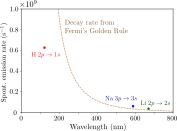
\includegraphics[width=0.53\textwidth]{emissionrates}
  \caption{Spontaneous emission rates (Einstein $A$ coefficients) for
    the $2p\rightarrow 1s$ transition in hydrogen, the
    $2p\rightarrow2s$ transition in lithium, and the $3p\rightarrow3s$
    transition in sodium.  Data points extracted from the NIST Atomic
    Spectra Database
    (\href{https://www.nist.gov/pml/atomic-spectra-database}{https://www.nist.gov/pml/atomic-spectra-database}).
    The dashed curve shows the decay rate based on Fermi's Golden
    Rule, with $|\mathbf{d}| \approx 10^{-10}\,\mathrm{m}$.  }
\end{figure}

%% Need to treat both electrons and photons on the same footing, with QFT
%% language.  Renormalization.

%% \section*{Exercises}

%% \begin{enumerate}
%% \item Gauge transformations.
%% \end{enumerate}

\section*{Further Reading}

\begin{enumerate}[[1{]}]
\item F.~J.~Dyson, \textit{1951 Lectures on Advanced Quantum Mechanics
  Second Edition}, arxiv:quant-ph/0608140. [\href{https://arxiv.org/abs/quant-ph/0608140}{link}]
\label{cite:dyson}

\item A.~Zee, \textit{Quantum Field Theory in a Nutshell} (Princeton
  University Press, 2010).
\label{cite:zee}

\item L.~L.~Foldy and S.~A.~Wouthuysen, \textit{On the Dirac Theory of
  Spin $1/2$ Particles and Its Non-Relativistic Limit}, Physical
  Review \textbf{78}, 29 (1950). [\href{https://journals.aps.org/pr/abstract/10.1103/PhysRev.78.29}{link}]
\label{cite:foldy}
\end{enumerate}

\end{document}


%% For decades after the discovery of quantum mechanics, the quantum
%% double-slit experiment was just a ``thought experiment'', meant to
%% illustrate the features of quantum mechanics that had been uncovered
%% by other, more complicated experiments.  Nowadays, the most convenient
%% way to do the experiment is with light, using single-photon sources
%% and single-photon detectors.  Quantum interference has also been
%% demonstrated experimentally using electrons, neutrons, and even
%% large-scale particles such as buckyballs.
